\section{Autonomous Taxi Fleet Model}
\label{sec:avmodel}

Based on the previously presented layers for the simulation of dynamic agents in
MATSim, a model for the specific case of autonomous vehicle taxi agents is developed
in the following sections. First, the general behavior is defined, which an AV agent needs to follow to serve a customer.
Furthermore, the questions of how to distribute AVs at the beginning of the simulation
and how to assign AVs to pending requests in an efficient manner are answered.
Finally, algorithms for routing AVs through the street network are presented and
evaluated.

\subsection{Agent behavior}

The behavior of an autonomous taxi is not a lot different from an ordinary one,
except that there is no need of random roaming to find new customers. Therefore,
the AV behavior presented here is mainly inspired by the model in \citet{Maciejewski2015}, where
ordinary taxi services have been simulated.

The behavior of an autonomous taxi agent can be described in terms of a task life
cycle. When the agent is not on a task, he is in idle mode, basically (for the basic
model) meaning that he will just stay at the current position and wait for further
instructions. The following steps in the life cycle are depicted in \cref{fig:avstates}.

\begin{enumerate}
\item \textbf{Pickup Drive} is the phase where the AV has got a task and is moving
to the requested pick up location. If the AV is already at the right location, this
point can be skipped. Otherwise, it represents a leg driving from the current position
to the pickup location.
\item \textbf{Waiting} is the phase in which the AV has arrived at the pickup
location, but the passenger is not there yet. This can only happen if passengers
request cars in advance, prior to the time when they want to be picked
up. If the passenger is already present at the time of the arrival at the pickup
location, this state can be skipped.
\item \textbf{Pickup} is the state in which the passenger is picked up. It is
modeled as a fixed time, e.g. one minute and starts as soon as both the AV
and the passengers are present at the pickup location.
\item \textbf{Dropoff Drive} represents the leg going from the pickup location to
the dropoff point.
\item \textbf{Dropoff} is the point where the passenger leaves the vehicle. Again,
this is modeled as a fixed time interaction.
\item \textbf{Idle} is the final (and initial) state of the AV life cycle. At this
point, the AV will just wait until it receives a new task to pick up another passenger.
\end{enumerate}

The states described above fit very well to the distinction of Activities and Legs
in MATSim as well as to the structure of the AgentFSM framework, which has been
developed for this purpose. Resulting from this behavioral model, a couple of
parameters and implementational questions arise, which must be configured accordingly:

\begin{description}
\item[The Idle behavior] for the basic model just means that the AV will stay at
its last position. Future extensions could make use of parking facilities or do
an intelligent repositioning to improve the overall performance of the service.

\item[Pickup and Dropoff duration] need to be specified. In accordance with
\citet{Bischoff2016}, $t_{pickup} = 120s$ and $t_{dropoff} = 60s$ have been chosen. The time
used for the pickup action will not be counted as waiting time (which, in turn,
would be penalized through the marginal utility of waiting as described in \cref{sec:utility}).
\end{description}

\begin{figure}
    \centering
    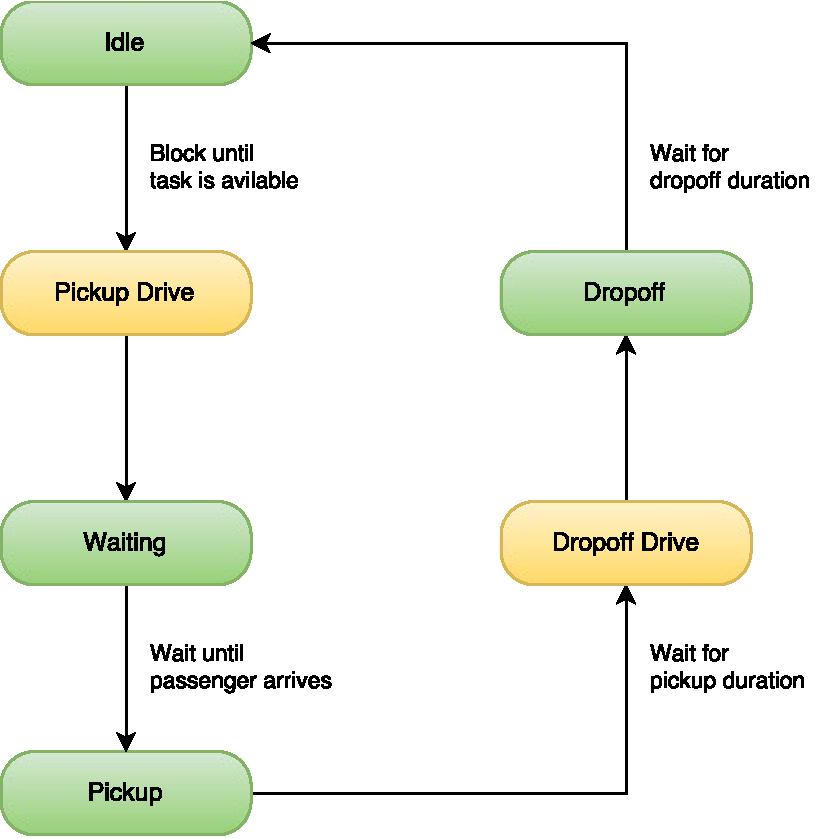
\includegraphics[width=0.7\textwidth]{figures/avstates.pdf}
    \caption{State chart of an AV agent. Activity states are displayed in green while Leg states are yellow.}
    \label{fig:avstates}
\end{figure}

\subsection{Distribution Algorithm}

At the beginning of a day simulation in MATSim, all the $n$ available AVs must be placed
somewhere in the network. Two simple distribution algorithms have been implemented
for the purpose of testing in this thesis.

The first one is \textbf{Random Distribution}. Here $n$ links are chosen randomly
from all available network links. While this is an easy distribution strategy for testing,
it creates a quite unrealistic scenario. Obviously, in a real AV service, vehicles
would be relocated overnight, such that they can serve as many passengers as
possible during the morning peek.

Therefore, a more elaborate distribution strategy has been implemented, which should
lead to more realistic results. One can define a density over the network,
such that every link has a certain probability to get an AV assigned. Then, in $n$
steps, the $n$ available AVs are added to a link dependent on the assignment
probability. This probability density can be based on many factors. The ones that are implemented
for this thesis are:

\begin{description}
\item[Population Density] The population density is measured in terms of
how many people are having their ``home'' activity on a certain link, since agents
will start their first simulated legs on a day from these locations. It should
be roughly related to the expected number of AV legs from that link.
\item[AV Density] For each link it is counted how many agents
have chosen the AV mode for their first leg (the one that is starting from home).
\end{description}

While the prior one is static, the latter on is dynamic in the sense that for every
iteration in the evolutionary learning, the density will change. So while the
population-density based distribution is a fixed constraint, the latter one captures
the factor of availability. For instance, if there are many agents using AVs in a
certain area, the availability is very high, and thus, more people might be inclined
to use it. On the other hand, if availability is low in an area, it might lead to
longer waiting times and people are less likely to use AVs.

While it might be interesting to observe different emerging patterns of availability,
the population density is better suited for the scope of this thesis. A
detailed investigation would need to be done if any results from the AV leg density
come from the mode choice of the agents or of feedback behavior within the algorithm
itself.

\subsection{Dispatcher Algorithm}

The dynamic dispatching of taxi vehicles is a complex scheduling problem,
which is hard to solve or needs numerous assumptions to be feasible. In
general, the problem will be NP-hard, and heuristical solution strategies need
to be applied if fast solutions are needed. An overview, as well as a proposed
heuristic algorithm, can be found in \citet{Maciejewski2015, Bischoff2016}.

The algorithm there can be described in two different states:

\begin{description}
\item[Oversupply] occurs when there are more available autonomous vehicles than
requests. This means that each request can be assigned without delay. In that case,
as soon as a request arrives at the dispatcher, the closest vehicle to this request
is searched and assigned to serve the customer.
\item[Undersupply] is the case when all autonomous vehicles are occupied. In that
case requests will stack up, which cannot be handled immediately. In this case the
algorithm works the other way round: As soon as an autonomous vehicle gets available,
it is dispatched to the closest request.
\end{description}

According to the beforementioned papers this strategy gives a near-optimal solution
with fast computational times.

The implementation for this thesis is based on a spatial relaxation of the traffic
network. This means that a grid with a specific resolution in x and y is fitted
over the links. One of these grids saves the locations of all the available AVs
while another grid saves the locations of all open requests. Because the grids have
a fixed structure, finding the closest AV or request is quite simple, since each
position in x and y belongs to one specific cell of the grid. If no option is found
in a certain cell, the search continues with all cells in its Moore neighborhood
(all eight surrounding cells). If this still gives no result, the radius is increased
and so forth. As soon as one or more candidates are found in a cell, a random one is
selected as the result of the search algorithm. This means that no further weighing
of the candidates is performed, which would lead to increased computation cost.
The procedure is depicted in \cref{fig:gridsearch}.

\begin{figure}
    \centering
    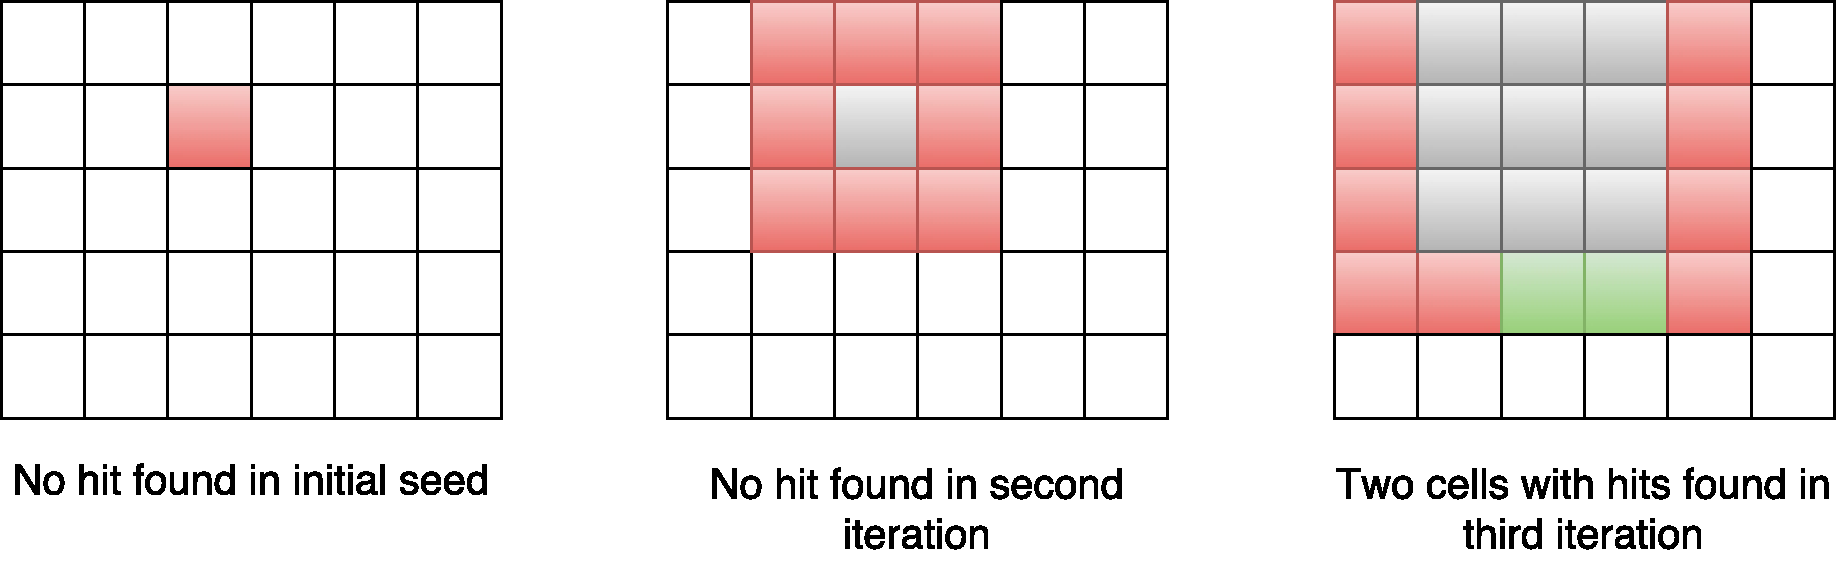
\includegraphics[width=1.0\textwidth]{figures/gridsearch.pdf}
    \caption{Schematic grid search algorithm for the dispatcher}
    \label{fig:gridsearch}
\end{figure}

This search algorithm imposes new parameters to the implementation, which
are the cell counts in horizontal and vertical direction. Depending on the topology
of the network, different parameters might be more efficient. If the grid is chosen
to be too dense, many iterations are needed in the algorithm, while a too sparse one
in the extreme case can lead to finding most of the items in only one single cell, effectively
transforming the to a simple random selection.

In fact, for some topologies, it might probably be more efficient to use different
data structures like a binary tree or quadtree to improve the search procedure.
Also, more elaborate network search algorithms could be used, which make direct use
of the topology \citep{ChenSpatial14}.

For the Sioux-14 scenario, it has been tested which impact the choice of the grid
size has on the results. In \cref{fig:gridsize} one can see, that very high-resolution
grids ($n=200$) lead to an increase in computational time, due to the necessary
``expansion'' of unoccupied cells, as described above. On the contrary, very low
grid sizes lead to poor results in terms of the overall average travel time of
the agents, because selecting a random agent from one of a few cells is
just a random assignment. A good value for the Sioux Falls network has been found to
be $n=20$, which is computed fast over the whole range of AV legs and furthermore
does a good job in decreasing the overall travel time.

\begin{figure}
    \centering
    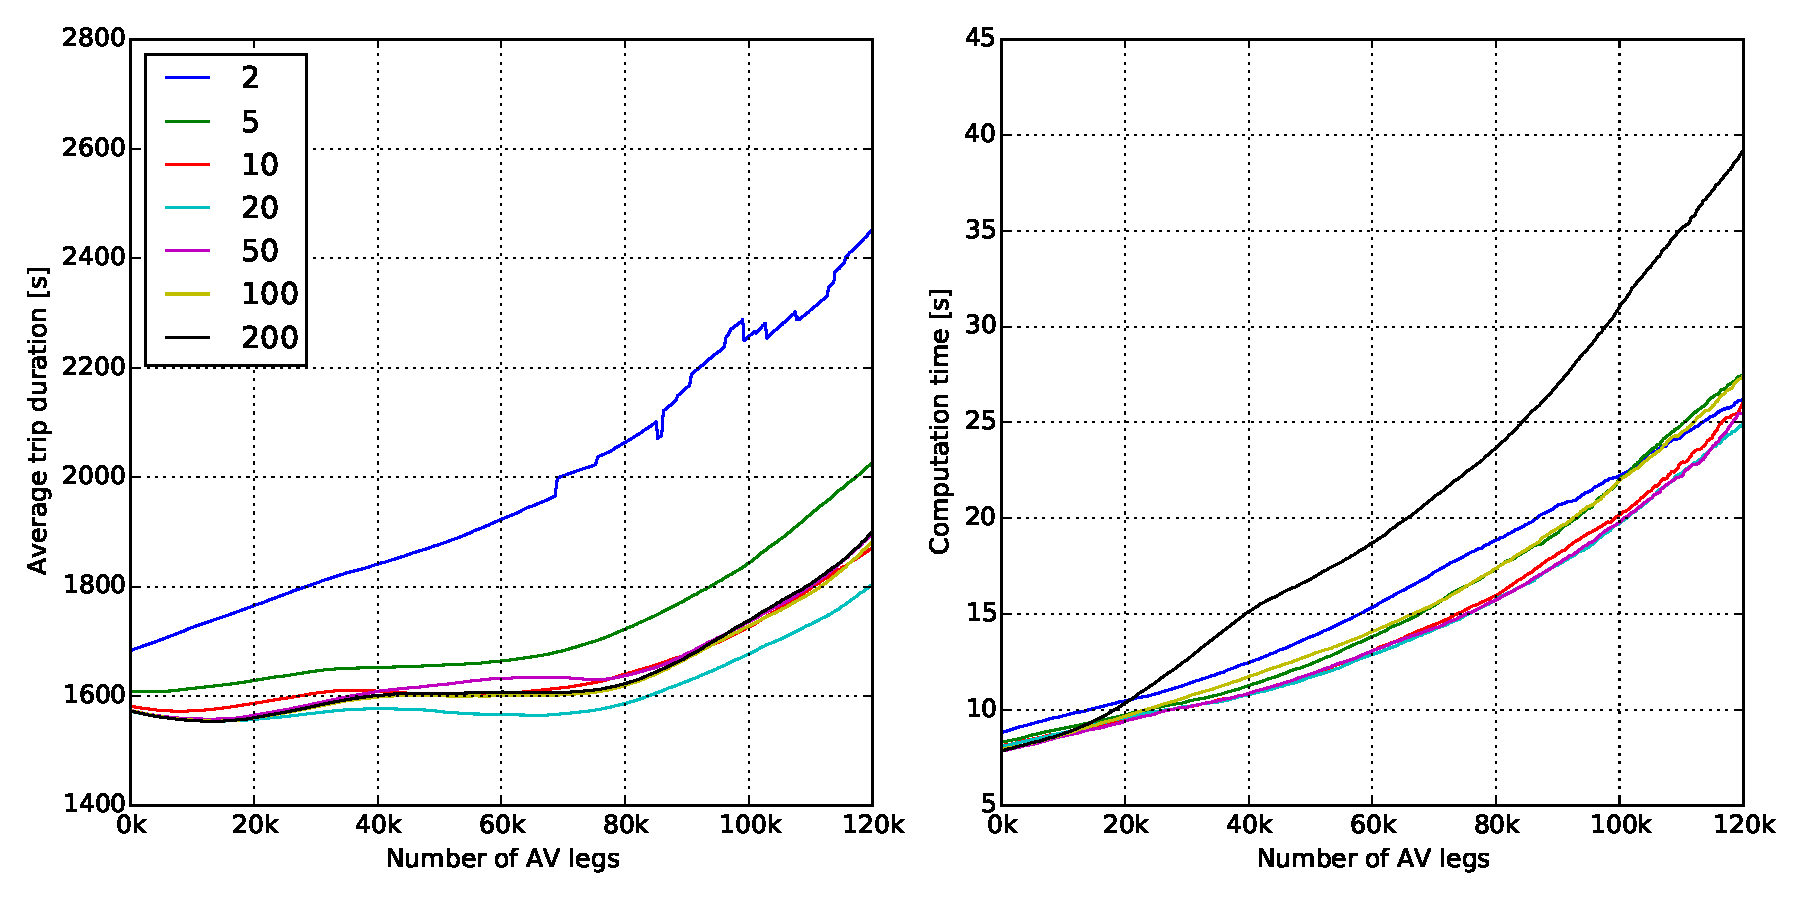
\includegraphics[width=0.9\textwidth]{figures/gridsize.pdf}
    \caption{Performance of different grid sizes in the dispatching algorithm for Sioux Falls}
    \label{fig:gridsize}
\end{figure}

Once one open AV request is assigned to one idle AV using these two grids, the
trip is computed, which mainly consists of finding a route for the AV to move
to the pickup location and finding a route from there to the dropoff point. The
actual implementation of this routing process will be described later (\cref{sec:routing}).

While in the first version of the dispatcher the routing was performed sequentially after
all trips had been assigned, the dispatching process could be improved by parallelizing
the routing stage with the whole QSim cycle as shown in \cref{fig:parallelrouting}.
At one point in the dispatcher, the assignments between requests
and AVs are made, just as before. Then, though, the actual task of finding the routes
is delegated to an arbitrary number of parallel routers. Each of those routers has
a queue which can be used to spread the routing tasks over all routers (i.e. if
there are two routers and six tasks, each one will process three tasks, which are
added to the respective queues). After all tasks have been sent to the routers,
the MATSim simulation continues as usual; the ``work-in-progress'' services are
saved temporarily in the dispatcher. After one whole QSim loop (i.e. simulating
the traffic network, static activities, ...) the dispatcher is called again. Then
it waits for all the routers to finally dispatch the requests that have
been assigned in the previous simulation step. Subsequently, the assignment step
for the current simulation step is performed.

\begin{figure}
    \centering
    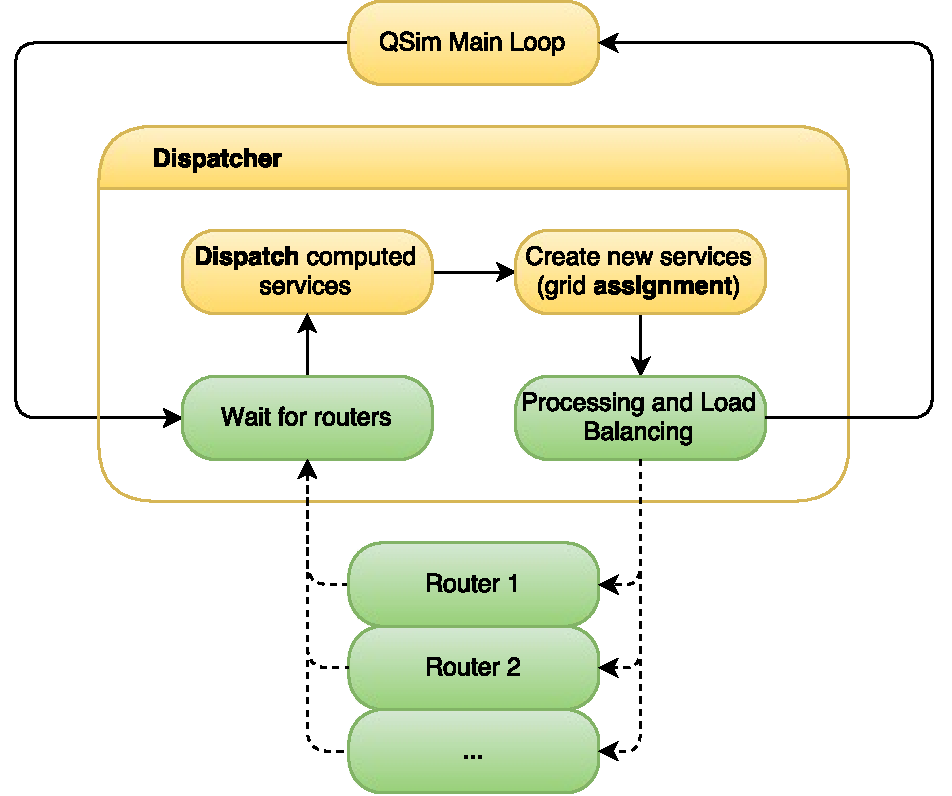
\includegraphics[width=0.9\textwidth]{figures/parallelrouting.pdf}
    \caption{Dispatcher implementation with routing parallel to the MATSim loop}
    \label{fig:parallelrouting}
\end{figure}

\Cref{fig:routers} shows the impact of adding this feature: Clearly, adding the
parallel functionality accounts for a significant decrease in computation time.
However, using more than one parallel router does not further increase the performance.
This is a strong indicator for the assignment step (together with the QSim) for
being the restricting time factor here. The routing of all tasks takes less time
than the other processes, even when only one router is present, and thus no further
gain in computation time can be made. Looking at the end of the graph, one can see
though that the offset in computation time that is accounted to the routing
is increasing faster than the computation time of the rest of the simulation. Therefore,
with a higher count of AV legs, there should appear the point where two routers
are more efficient than one.

In theory, the parallelization of the dispatcher could be pushed even further.
However, the assignment step, which is the other expensive component in the algorithm,
would probably be hard to parallelize because concurrent workers
would need to access the same grid structures. The overhead of managing which
worker has access is likely to add more overhead than improvement to
the simulation quickly. One could, however, put the whole assignment process as a serial
procedure in parallel to the QSim, as done with the routers. This could be a
promising approach to decreasing the computation time even further.

\begin{figure}
    \centering
    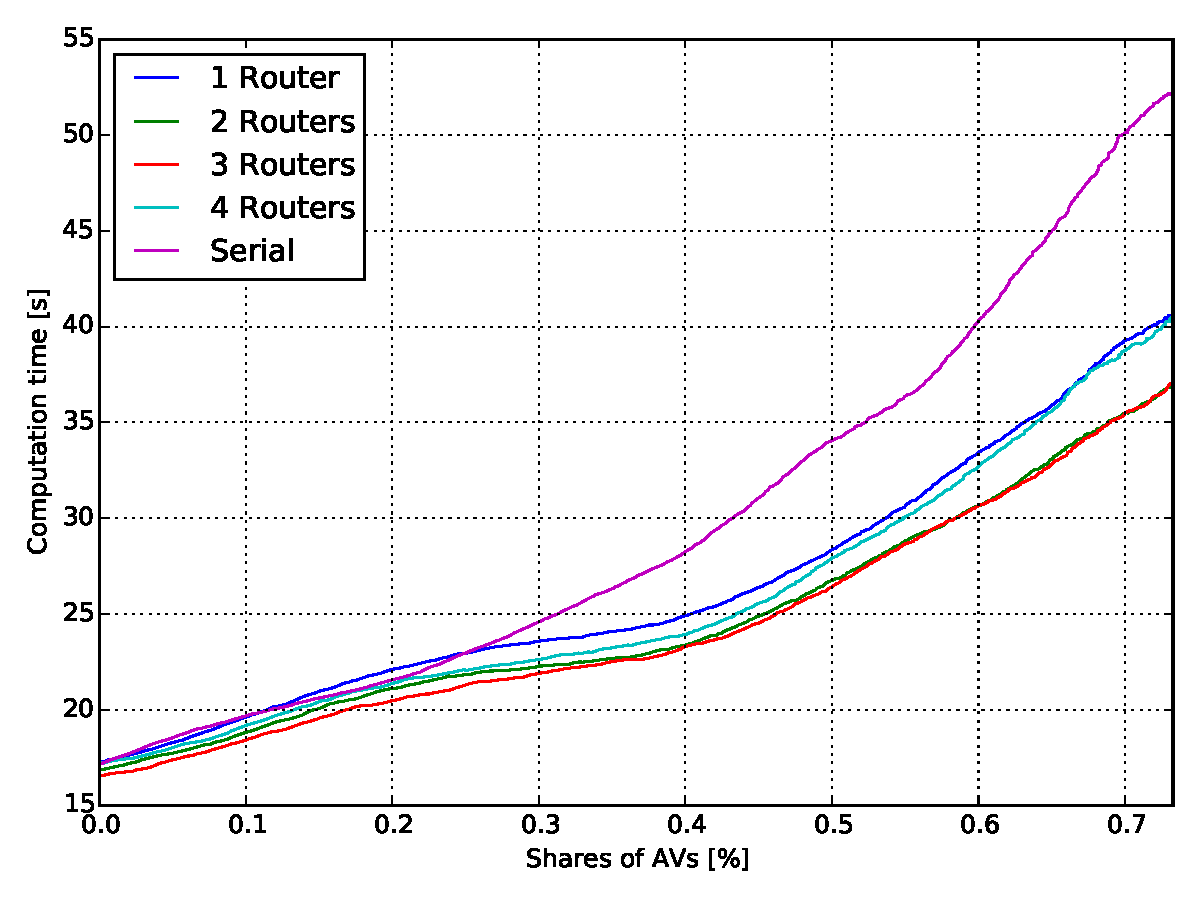
\includegraphics[width=0.9\textwidth]{figures/routers.pdf}
    \caption{Computational performance of the dispatcher with sequential and parallel routing}
    \label{fig:routers}
\end{figure}

\subsection{Routing Algorithm}
\label{sec:routing}

The routers in the AV simulation have the task to find a route through the street
network. For each AV service, there are two of such routes: The pickup route from
the AV's current position to the customer and the drop off route on which the customer
is transported to the predefined drop off location. To find the routes, the Dijkstra algorithm is used \citep{Dijkstra}, with
travel time as the objective to be minimized. This travel time is computed using
the length of the selected links and the speeds on those links.

The most simple idea for those speeds, however, would be to use the predefined free-flow speed values in
the scenario network. While this approach works for small shares of AVs, it leads
to heavy overcongestion with high numbers of AVs on the streets. The reason
for this is that for similar trips, similar routes are chosen, leading AVs to make
extensive use of the main arterials, but also of specific low-capacity links, which
are optimal for topological reasons. By not taking into account any information
on how congested the links are, more and more vehicles attempt to enter
them, creating huge traffic jams.

In the top-level MATSim loop, such congestion can mainly be  avoided by introducing
small stochastic and congestion-based alterations to the car-using agents. This way,
iteration by iteration, such routes are eliminated from their plans because they
lead to a bad scoring of the respective plans. Furthermore, the traffic situation
by daytime in the network is measured and used as a basis for planning in subsequent
iterations.

In the following sections, two more advanced approaches for defining the link speeds
are presented. First, continuous online tracking of link speeds during the day is
discussed in \cref{sec:routing_online}, followed by an approach based on the
introduction of stochasticity into the process (\cref{sec:routing_variation}).

The problem of routing \textit{all} vehicles in a network (which is
in principal the case for very high shares of the AV mode), is a complex problem
in itself. In this perspective, the presented routing algorithms are versions of
a local optimization of the route for each agent and trip. However, this does in
no way guarantee that a global optimum is reached (depending on what the objective
is). In that regard global routing algorithms and heuristics might be worth to study in the future.

\subsubsection{Online Speed Calculation}
\label{sec:routing_online}

One approach that has been tested for the routing is to base the link speeds on
actual online measurements in the network. The traffic situation on
a link can be described by the three interconnected measures flow,
density and speed. Flow describes the throughput of the link, i.e. at the start
or the end of the link it is measured how many vehicles cross that link in a
certain time interval while the density describes how many vehicles are on
the link at a certain time.

Each link in MATSim has a certain flow capacity $q_c$ in $\left[\frac{veh}{h}\right]$ defined, stating the maximum number
of cars per hour, that are allowed to pass the link.
Furthermore, for each link it can be counted how many cars are on the street by
counting the number of cars going in $n_{in}$ and out $n_{out}$, whenever either
event happens. This allows one to computed the density on the link:

\begin{equation}
d = \frac{\Delta n}{l} = \frac{n_{in} - n_{out}}{l}
\end{equation}

with $l$ being the length $[km]$ of the respective link. These values can be combined
to arrive at the current link speed by computing:

\begin{equation}
v = \frac{q_c}{d} = \frac{q_c \cdot l}{\Delta n}
\end{equation}

The result is a velocity in $\left[ \frac{km}{h} \right]$.
It states the maximum possible speed when a certain density $d$ appears on
a link with the maximum flow capacity of $q_c$.

Of course, computing this value might lead to speeds, which exceed the predefined
maximum free-flow speed of the link, so the final value is bounded from above. Also,
for the proper working of the Dijkstra algorithm, a minimum speed is defined to
$1 \frac{km}{h}$:

\begin{equation}
v' = \begin{cases}
1 \frac{km}{h} & \text{if } v < 1 \frac{km}{h} \\
v & \text{else } \\
v_f & \text{if } v > v_f
\end{cases}
\end{equation}

In order to avoid the same computation whenever a link should be traversed, the
network is computed collectively after a fixed time span, e.g. every $30s$ in
simulation time.

\subsubsection{Stochastic Variation Model}
\label{sec:routing_variation}

The second idea is to add stochasticity to the Dijkstra process, thus creating
slightly perturbed routes. What needs to be answered for using this approach is,
which magnitude those perturbations should have. To solve this problem,
the Sioux-16 baseline scenario has been examined. The 30h day has been divided
into $N=720$ bins ($2min$ each) and for each the relative decrease in speed for
all link passages starting has been computed:

\begin{equation}
r_{i,j} = \frac{1}{n_i} \sum_{j=1}^{n_i} \frac{v_{i,j,free-flow} - v_{i,j,simulation}}{v_{i,j,free-flow}}
\end{equation}

Here $n_i$ is the number of link passages (all agents and all links) that occurred
in bin number $i$ and $r_{i,j}$ is the relative decrease of speed in each bin for
each passage.

As can be seen in \cref{fig:speeddecdist}, the distribution of decreases in travel
speeds of the network links can roughly be approximated using a Gamma distribution. The outliers,
which can be seen on the right, are those cases where there is a much congestion during
peak hours. Because those are exactly the cases that one wants to avoid here, they
are omitted in the following steps.
The assumption of a Gamma distribution is wholly motivated by the shape of the histogram,
performing an educated derivation of the distribution shape would be an interesting
investigation, which is out of the scope of this thesis.

A Gamma distribution is defined by a shape parameter $k$ and a scale parameter $\theta$. For
all bins in the baseline scenario, the respective parameters have been obtained using
the MLE estimator for $\theta$ and a Newton approximation for $k$ as described in
\citet{Minka2002}. \Cref{fig:randommodel} shows the parameter values for each bin on top,
after they have been smoothed using a moving average filter of length $20$. Also,
for the times before roughly 5 am and after 10 pm, average parameter values over the
off-peak hours in the middle of the day have been inserted due to a lack of sufficient
data for fitting the speed decreases in these outer areas.

Also shown in \cref{fig:randommodel} (on the bottom) is the mean of the speed decrease at each time of the
day, framed by the $10\%$ and $90\%$ quantiles, now instead of simulation results based on the statistical model.
It can be seen that due to the Gamma model, the range of probable decreases is high during peak hours, up to 70\%,
while the 10\% stays quite constant during the day. The graph of the mean suggests that the presented
model is a reasonable approximation, which qualitatively makes sense.

The final travel speed for the router can now be described as a random variable:

\begin{equation}
    V_{i,j,routing} = v_{i,j,free-flow} \cdot (1 - \text{min}\{ R_i, 1 \})
\end{equation}

with $R_i \sim \Gamma(k_i, \theta_i)$ being Gamma-distributed for each bin.

The overall effect of this model is then as follows: There is a certain increase
in travel time expected for each link, which depends on its free-flow speed and the time
of the day. However, especially during peak hours, when the bottlenecks would be a
critical problem, more variation is added to the expected increases in travel time
and thus a better variation in the routing is reached.

The expected increases are founded on the actual network characteristics of the Sioux-16 network
and might be different for other networks. Furthermore, it has not been investigated
whether different link types might show different statistical properties, which
is very likely. Establishing a comprehensive statistical model of the decreases
in link speeds, depending on a greater variety of variables, would be beneficial.

\begin{figure}
    \centering
    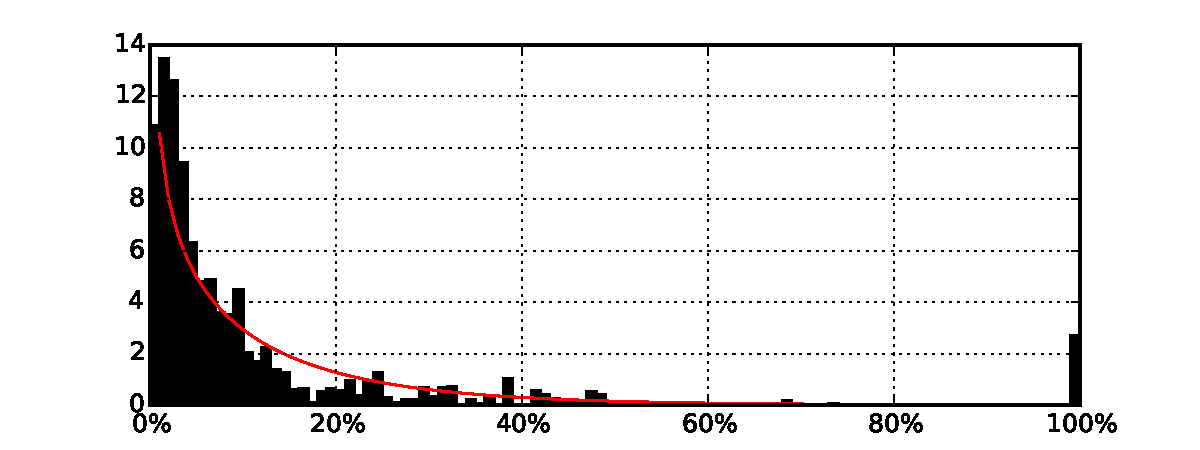
\includegraphics[width=0.9\textwidth]{figures/speeddecdist.pdf}
    \caption{Example distribution (pdf) of relative decreases in link speed}
    \label{fig:speeddecdist}
\end{figure}

\begin{figure}
    \centering
    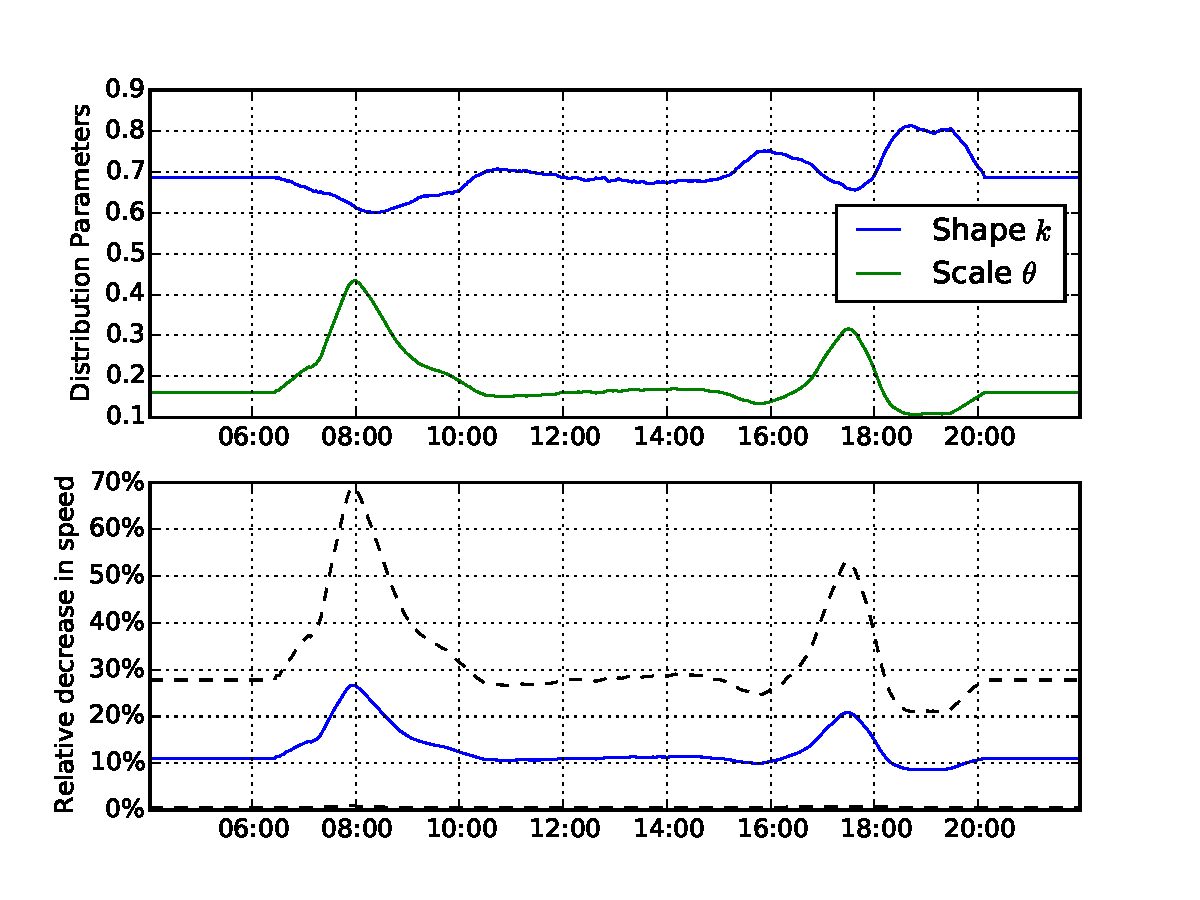
\includegraphics[width=0.9\textwidth]{figures/randommodel.pdf}
    \caption{Statistic model for the relative decrease in link speed. Top: Parameters
    for the Gamma distribution model by day time. Bottom: Mean value of the respective
    Gamma distribution and the 10\% and 90\% quantiles.}
    \label{fig:randommodel}
\end{figure}

\subsubsection{Performance Measures}
\label{sec:routingperf}

Basic tests of the AV taxi fleet model without the evolutionary replanning have been performed to test the
performance of the routing algorithms. For that purpose, the scenario has been
simulated for one iteration, without any further refining of the agent plans.
First, the plans of 30\% of the agents using a car in the population have been
changed to use AVs. \Cref{fig:relaxed_routing_fraction} shows how
the average travel time in the network changes with an increasing number of AVs.
If only a few AVs are available, the waiting time for an AV is very high, because
there are not enough vehicles to cover the demand. With an increasing number of
available AVs the congestion in the network increases and therefore the average
travel time (of cars) in the network increases. Clearly, the online speed tracking performs
better in preventing congestion while the Gamma distribution approach shows a
similar performance to a simple routing based on the free-flow speed.

Another case is presented in \cref{fig:relaxed_routing_supply}. There the number
of available AVs has been fixed to 2000, and different shares of AV trips in the
population have been examined. In that dimension that waiting time increases with
a higher share of the population, since more demand is generated, which the taxi
service is less and less likely to cover the more agents are using it.
Interesting is the decrease in overall travel time, which occurs because at some
point the number of waiting people exceeds the number of people on the road, which
is freeing the network from congestion, while letting people wait for
a much longer time.

Finally, while the former cases were ``relaxed'' in the way that although leading
to high waiting times, the demand could be covered in the 30h simulation day, \cref{fig:routing_constrained}
shows the case were this is not the case anymore. In that figure, 70\% of all car
trips have been replaced by AV trips. The solid lines show the average travel time
of cars in the network for cases in which all agents could finish their plans; the
dotted lines indicate cases where agents were not able to do so. In the beginning
of the graph, for a very low number of AVs, all algorithms break down in this
regard. This is due to the disability to serve the demand with that number of
vehicles.

For the online calculation approach, one can see, that it is performing badly
throughout the whole range of values. One explanation for that
is that AVs react to any slowdown in the network, effectively trying to find alternative
routes to prevent them. This leads the AVs to find unnecessarily long trips, which
take irrational routes through the network. What is missing in this routing approach
is a sense of expected congestion. In a network, where the capacity of the roads is
not able to allow for a free flow at all times, the routing algorithm should
be able to bargain between joining a traffic jam and expecting it to dissolve soon
or choosing a completely different route through low-capacity links. In this approach,
the latter will lead to even more severe congestion because those links are used
more frequently than would be necessary.

Comparing the free-flow speed router and the stochastic one, the performance is similar.
There is a gap in the middle of the graph, showing the area in which too much
congestion is produced by the AVs, such that agents get stuck. Before the gap,
one has the regime where AVs serve multiple requests
since there are not enough AVs available to have one AV for each request. Then,
if the number of AVs gets bigger, it happens that because more and more users get
their ``unique'' AV, more cars go on the street, and too much congestion occurs.
Finally, if there are even more AVs, the situation relaxes again, because now
almost every request has it's own car. There is no need to perform additional
pickup trips to the customers since there are enough AVs distributed over the
network.

The gaps presented in this scenario are likely to be resolved when the evolutionary
replanning is introduced into the model. Because people can reschedule
their departures, the situation can be relaxed. Also in the replanning, agents would
choose other means of transport if the use of AVs gets to disadvantageous. However,
it has been found that also with the replanning, for some scenarios it occurs that
not all agents arrive at the end of the day. As can be seen in \cref{fig:routing_constrained},
the stochastic approach can cover a larger range of cases, and it also has
been found that in combination with the replanning, this approach yields the strongest
reliability. Therefore, it is chosen in the following simulations of the whole
model.

\begin{figure}
    \centering
    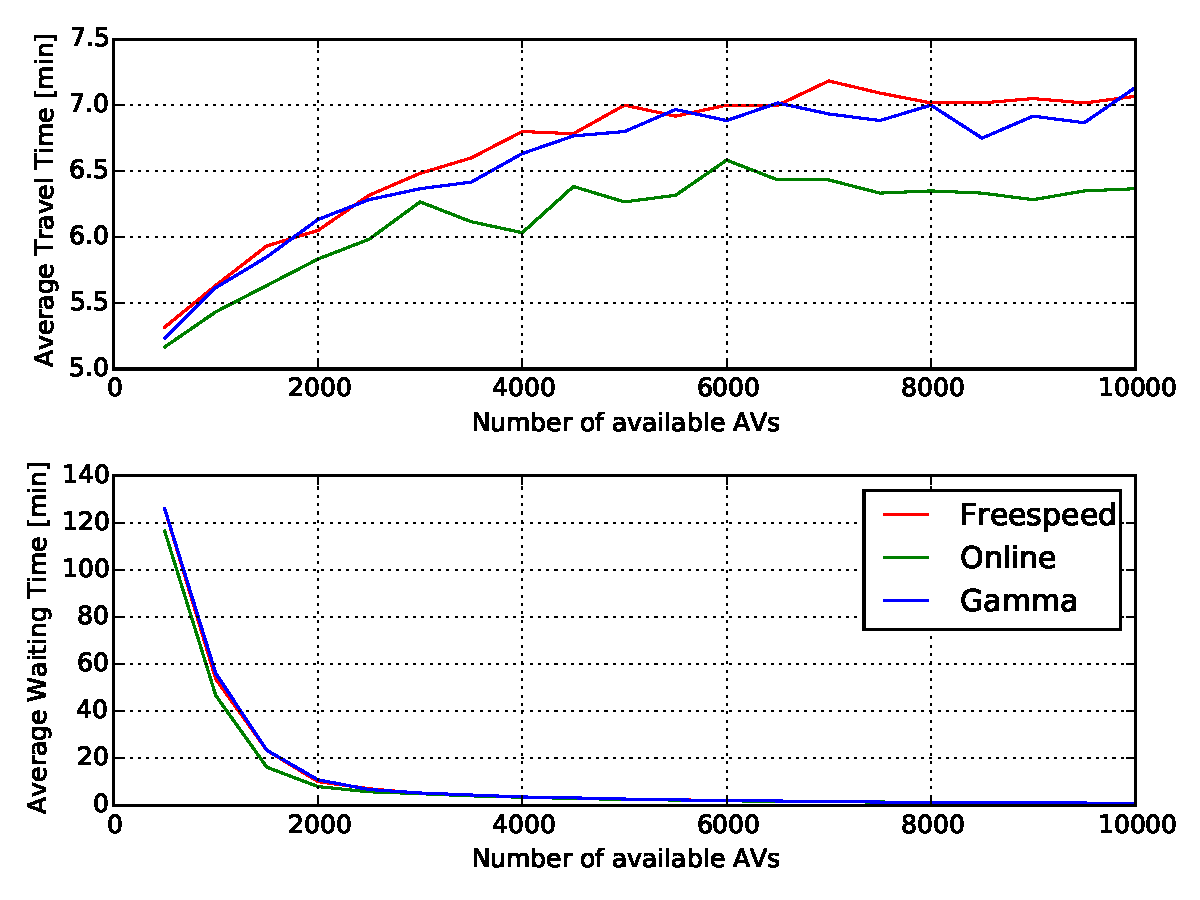
\includegraphics[width=0.9\textwidth]{figures/relaxed_routing_fraction.pdf}
    \caption{Comparison of different routing algorithms in terms of average travel time and average
    waiting time with a fixed share of 30\% of car users in the population using AVs.}
    \label{fig:relaxed_routing_fraction}
\end{figure}

\begin{figure}
    \centering
    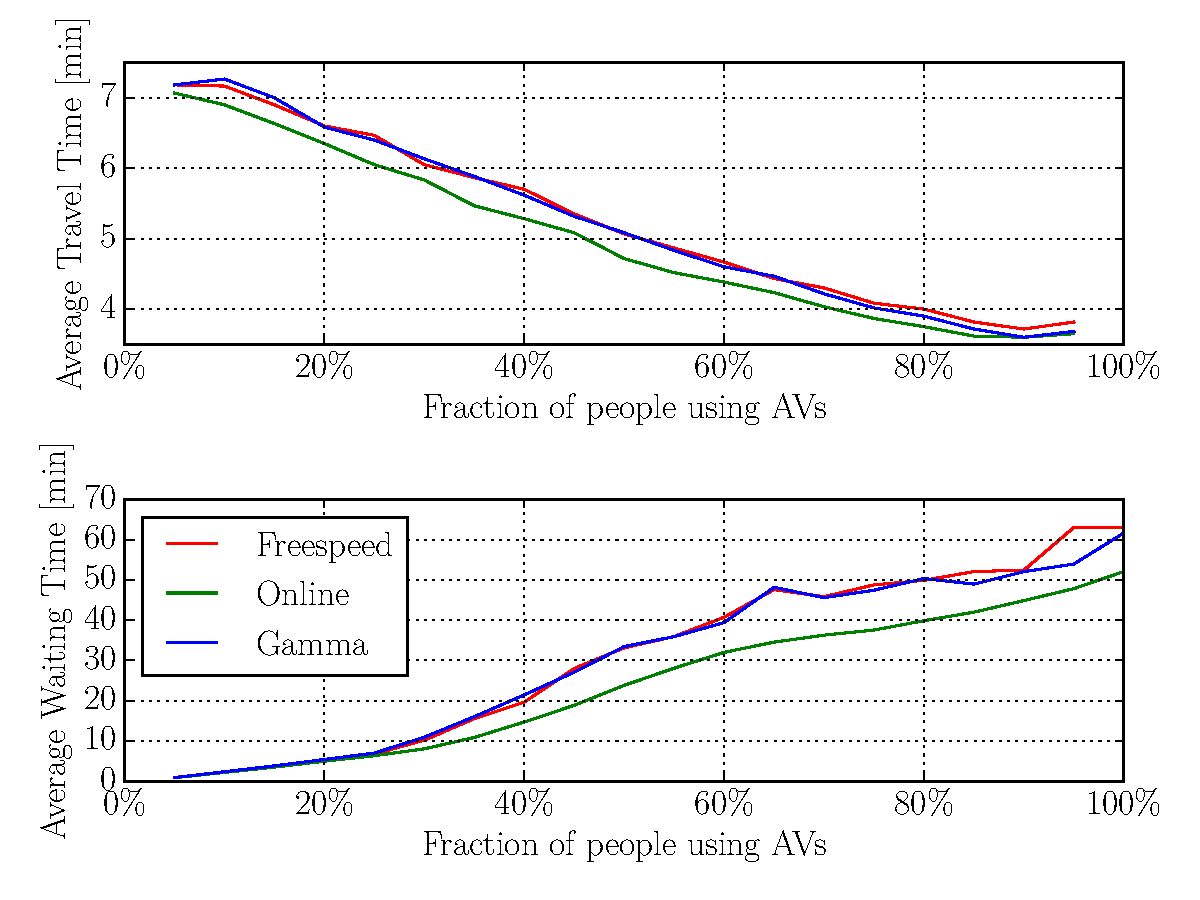
\includegraphics[width=0.9\textwidth]{figures/relaxed_routing_supply.pdf}
    \caption{Comparison of different routing algorithms in terms of average travel time and average
    waiting time with a fixed number of 2000 available AVs.}
    \label{fig:relaxed_routing_supply}
\end{figure}

\begin{figure}[h]
    \centering
    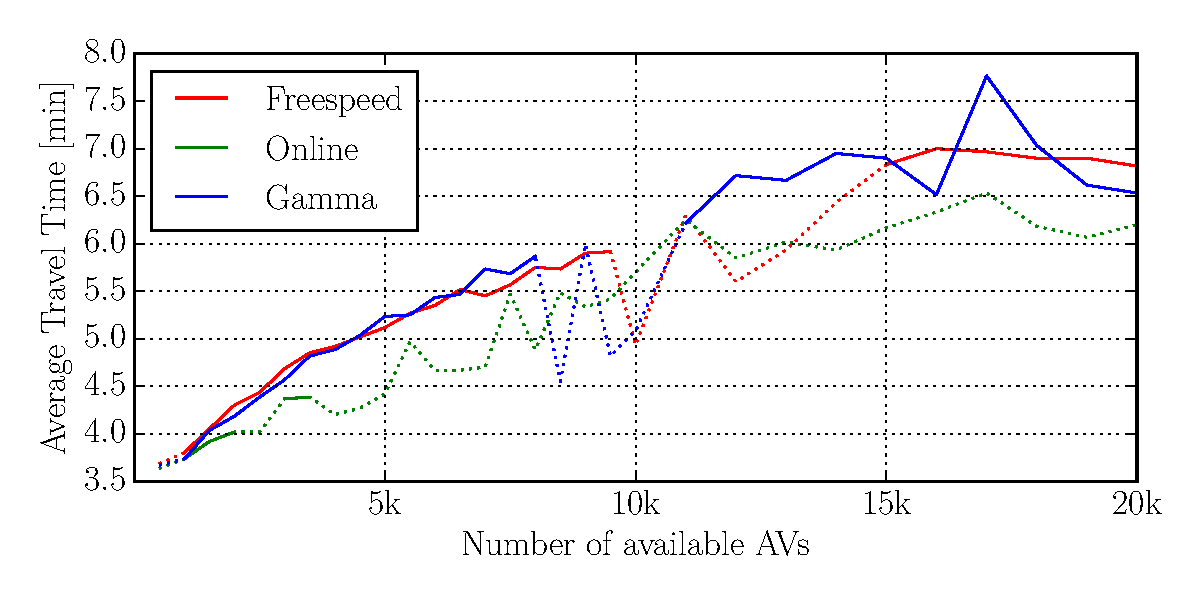
\includegraphics[width=0.9\textwidth]{figures/routing_constrained.pdf}
    \caption{Comparison of different routing algorithms in terms of average travel time with a fixed share of 70\% of car users in the population using AVs.
    Dotted lines show areas where agents were not able to finish their plans during the 30h simulation period.}
    \label{fig:routing_constrained}
\end{figure}

\FloatBarrier
\subsubsection{Static Trip Replacement}
\label{sec:replacement}

From the data for the stochastic routing, it was possible to find a structured
dependency of the number of available AVs and the number of replaced cars in
terms of the waiting time for passengers without performing any additional measurements.
The result is presented in \cref{fig:replacementwaiting}. There, the existing data
points are depicted as crosses, while all combinations with an average passenger
waiting time of less than 10min have been highlighted. A pareto front over the
existing measurements has been constructed. So in the case of a bare replacement
of car trips by AV trips, one can see that in order to replace 40\% of the car fleet,
10,000 AVs are necessary to reach the desired waiting time, which is only 15\% of
the cars in the baseline scenario. So in total one would be left with a total car and
av fleet size of 75\%. In the case of a replacement of 70\% of private cars with
AVs, one would need to convert 30\% of vehicles to AVs, which would yield a
total fleet size of 60\%.

Furthermore it should be mentioned, that taking the average as a waiting time
threshold might yield misleading results, i.e. if the distribution is heavily
biased towards low waiting times. Experiments with using quantile functions instead
of the average showed that in fact the opposite case is observed here. The shown
average coincides quite accurately with the 80\% quantile, thus yielding an answer
to the more solid question: How many AVs are needed to replace a certain percentage
of the initial car fleet if 80\% of the waiting times should be less than 10
minutes.

These results are a first indicator of the performance of the model, but of course
lack the flexibility of the evolutionary replanning. By letting agents alter their
departure times the demand situation should become more relaxed and therefore
waiting times should decrease. This, in turn would mean that the displayed front
would decrease in slope. The next section will cover the results gained from the
combined simulation framework, where all components are added together.

\begin{figure}
    \centering
    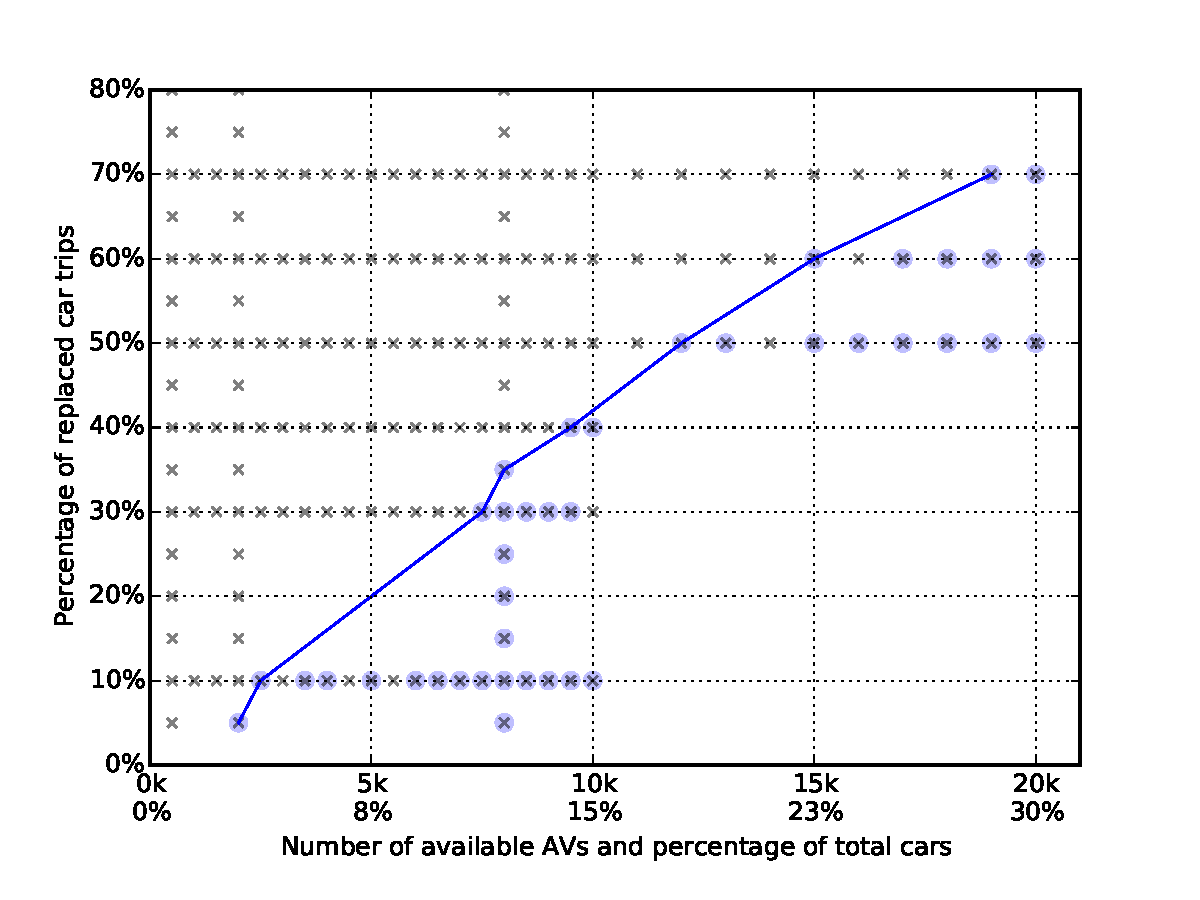
\includegraphics[width=0.9\textwidth]{figures/replacementwaiting.pdf}
    \caption{Dependency of the number of available AVs and the number of replaced
    cars. The crosses indicate distinct measurements; the highlighted ones yield
    an average passenger waiting time of less than 10 minutes.}
    \label{fig:replacementwaiting}
\end{figure}
